\documentclass{article}
\usepackage[utf8]{inputenc}
\usepackage[russian]{babel}
\usepackage{graphicx}
\usepackage{amsmath}
\usepackage{breqn}
\usepackage{wrapfig}
\usepackage{float}
\usepackage{multirow}
\usepackage{caption}
\usepackage{subcaption}

\graphicspath{ {./data/images} }
\author{Александр Романов Б01-107}
\date{}
\title{4.3.2. Дифракция света на ультразвуковой волне в жидкости. (А. Вертикальная щель)}

\begin{document}
\maketitle
\section{Введение}
\subsection{Цель работы}
Изучение дифракции света на синусоидальной акустической решётке и наблюдение фазовой решётки методом
тёмного поля.
\subsection{В работе используются}
Оптическая скамья, осветитель, два длиннофокусных объектива, кювет с жидкостью, кварцевый излучатель с
микрометрическим винтом, генератор ультразвуковой частоты, линза, вертикальная нить на рейтере, микроскоп.
\section{Работа}
\subsection{Определение скорости ульразвука по дифракционной картине}
Соберём схему на Рис. \ref{fig:difr-scheme}.

\begin{figure}[H]
  \centering
  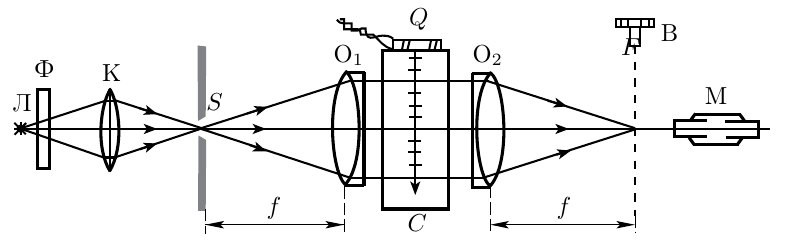
\includegraphics[width=\textwidth]{difr-scheme.png}
  \caption{Схема наблюдения дифракции на акустической решётке}
  \label{fig:difr-scheme}
\end{figure}
Фокусные расстояние объективов \(O_1\) и \(O_2\) одинаковы (\(f = 30\; cm\)), поэтому хд лучей в системе
получился симметричным.

Ярко осветим щель с помощью кондесора. Предварительную настройку будем проводить с зелёным фильтром.
Убедимся что световое пятно на щели равномерно освещено. Затем с помощью листа бумаги найдём резкое
изображение щели \(S\) в фокальной плоскости объектива \(O_2\) (на самом деле примерно \(35\; cm\)).
Настроим микроскоп на отсчётное устройство. Получим в поле зрения микроскопа систему дифракционных
полос.
\begin{figure}[H]
  \centering
  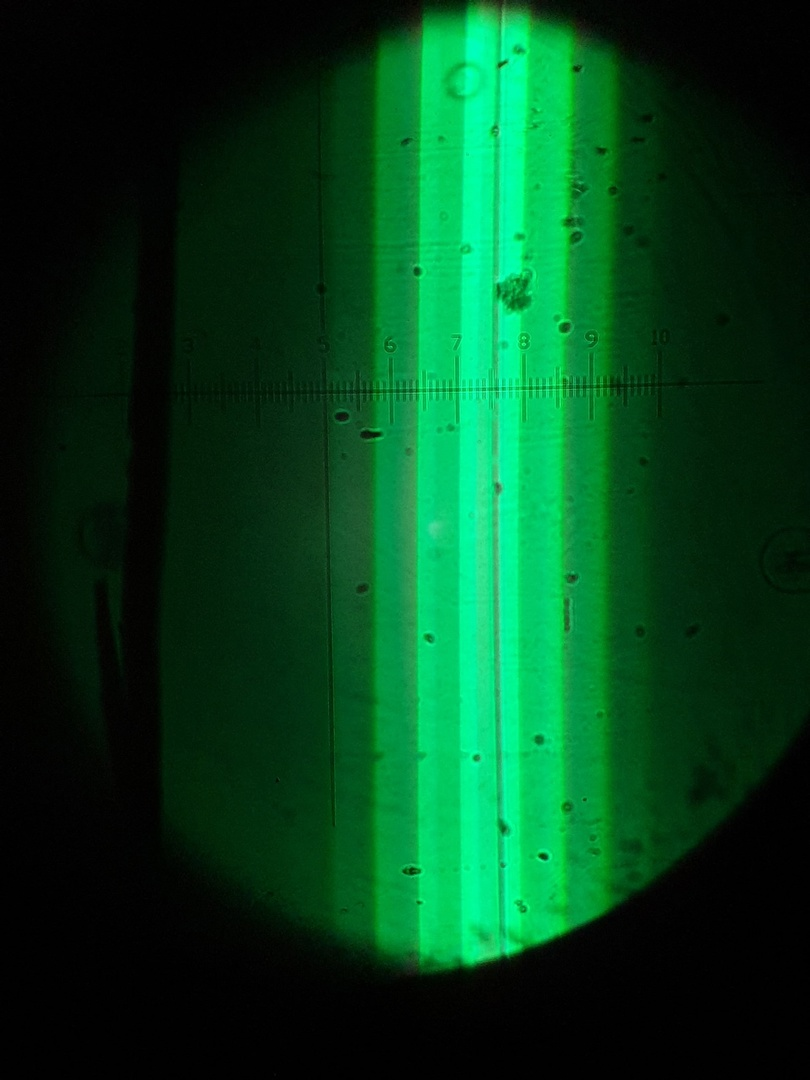
\includegraphics[width=0.5\textwidth]{green-lines.jpg}
  \caption{Зелёные дифракционные полосы}
  \label{fig:green-lines}
\end{figure}

Заменим широкополосный зелёный фильтр красным. Изменяя ширину щели \(S\), её наклон и положение конденсора
добьёмся оптимальных условий наблюдения дифракционных полос. 

При увеличении частоты ультразвука полосы то появляются, то исчезают. При это из количество и расстояния 
между ними увеличивается. Ширина самих полос остаётся неизменной.

Перемещая излучатель с помощью микрометрического винта, оценим длину УЗ-волны как удвоенное расстояние
между наиболее чёткими дифракционными картинами:
\[ \lambda = 2 \pm 0.01\; mm \]
Определим скорость звука в воде (\(f = 1.2 \pm 0.05\; MHz\)):
\[ c = \lambda \cdot f = (2400 \pm 700)\; m/s\] Несмотря на то, что погрешность большая это совпадает с табличным
значением \(c = 1500\; m/s \) в пределах погрешности.

Для той же частоты (\(f = 1.2 \pm 0.05\; MHz\)) определим положения \(x_m\) семи дифракционных максимумов
с помощью микрометрического винта отсчётного устройства (по перекрестию).
Фильтр: \(\lambda  (6400 \pm 200) \cdot 10^{-10}\; m\)
\subsection*{\(f = 1.2 \pm 0.05\; MHz\)}
\begin{figure}[H]
  \centering
  \begin{tabular}{|c|c|c|c|c|c|c|c|}
    \hline
    \(m\) & 0 & 1 & 2 & 3 & 4 & 5 & 6\\\hline
    \(x_m,\; (1 \pm 4) \mu m\) & 160 & 320 & 464 & 620 & 780 & 940 & 1080\\\hline
  \end{tabular}
  \caption{\(f = 1.2\; MHz\)}
\end{figure}

Построим график \(x_m\) от \(m\):
\begin{figure}[H]
  \centering
  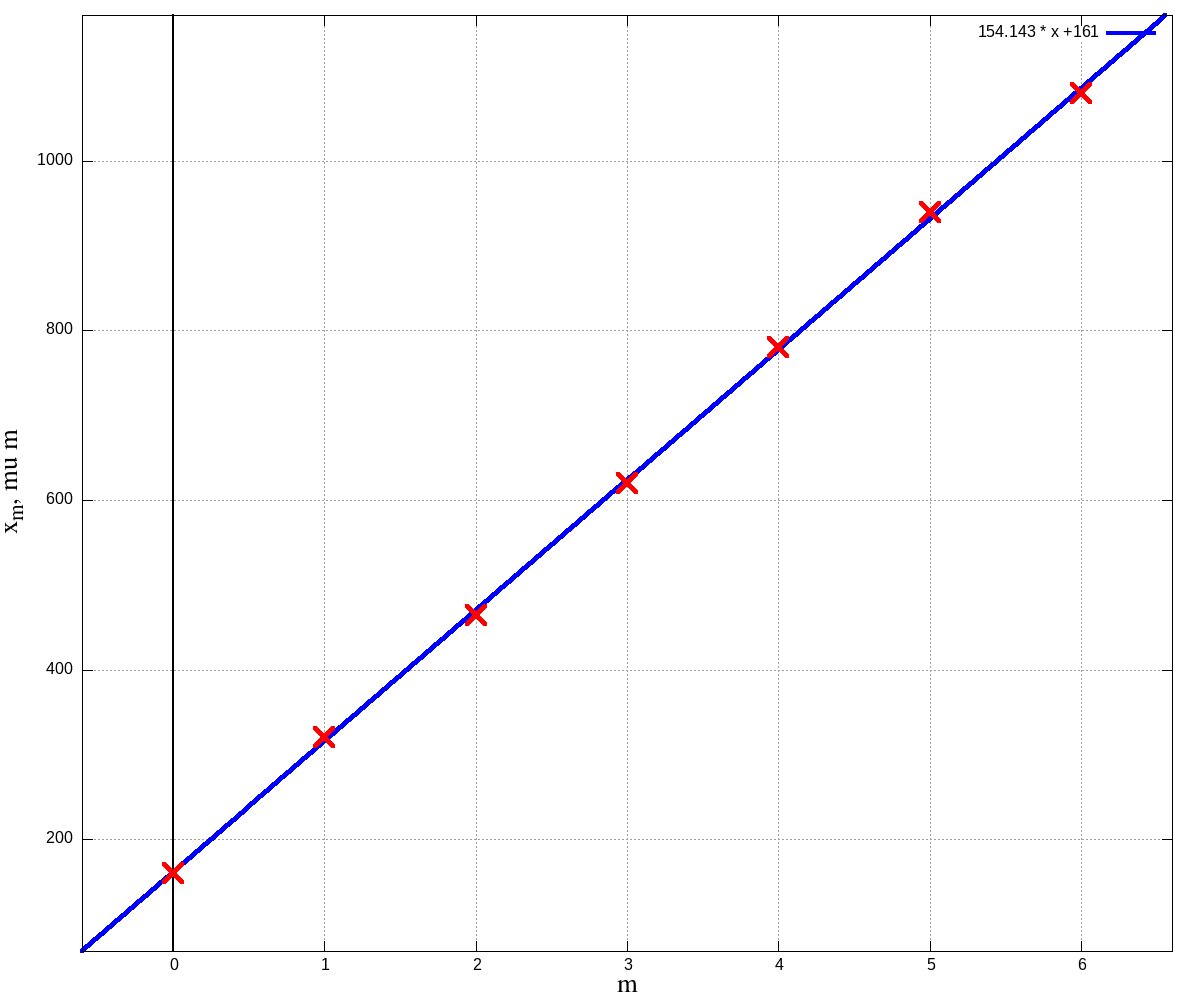
\includegraphics[width=\textwidth]{1200KHz.png}
  \caption{График \(x_m\) от m для \(f = 1.2\; MHz\)}
  \label{fig:1200KHz}
\end{figure}

Получили зависимость вида \(y = kx + b\):
\[ k = (154 \pm 5)\; \mu m \]
\[ b = (161 \pm 6)\; \mu m \]
Из углово-го коэффициента получим, что расстояние между соседними полосами равно:
\[ \Delta x = (154 \pm 5)\; \mu m \]

Т.к. 
\[ l_m = mf\frac{\lambda}{\Lambda} \]
то:
\[ \Lambda = \frac{f\lambda}{\Delta x} = 1247 \pm 16 \]

Повторим для других частот:

\subsection*{\(f = 1.14 \pm 0.005\; MHz\)}
\begin{figure}[H]
  \centering
  \begin{tabular}{|c|c|c|c|c|c|c|c|}
    \hline
    \(m\) & 0 & 1 & 2 & 3 & 4 & 5 & 6\\\hline
    \(x_m,\; (1 \pm 4) \mu m\) & 186 & 320 & 464 & 616 & 772 & 900 & 1140\\\hline
  \end{tabular}
  \caption{\(f = 1.14\; MHz\)}
\end{figure}

Построим график \(x_m\) от \(m\):
\begin{figure}[H]
  \centering
  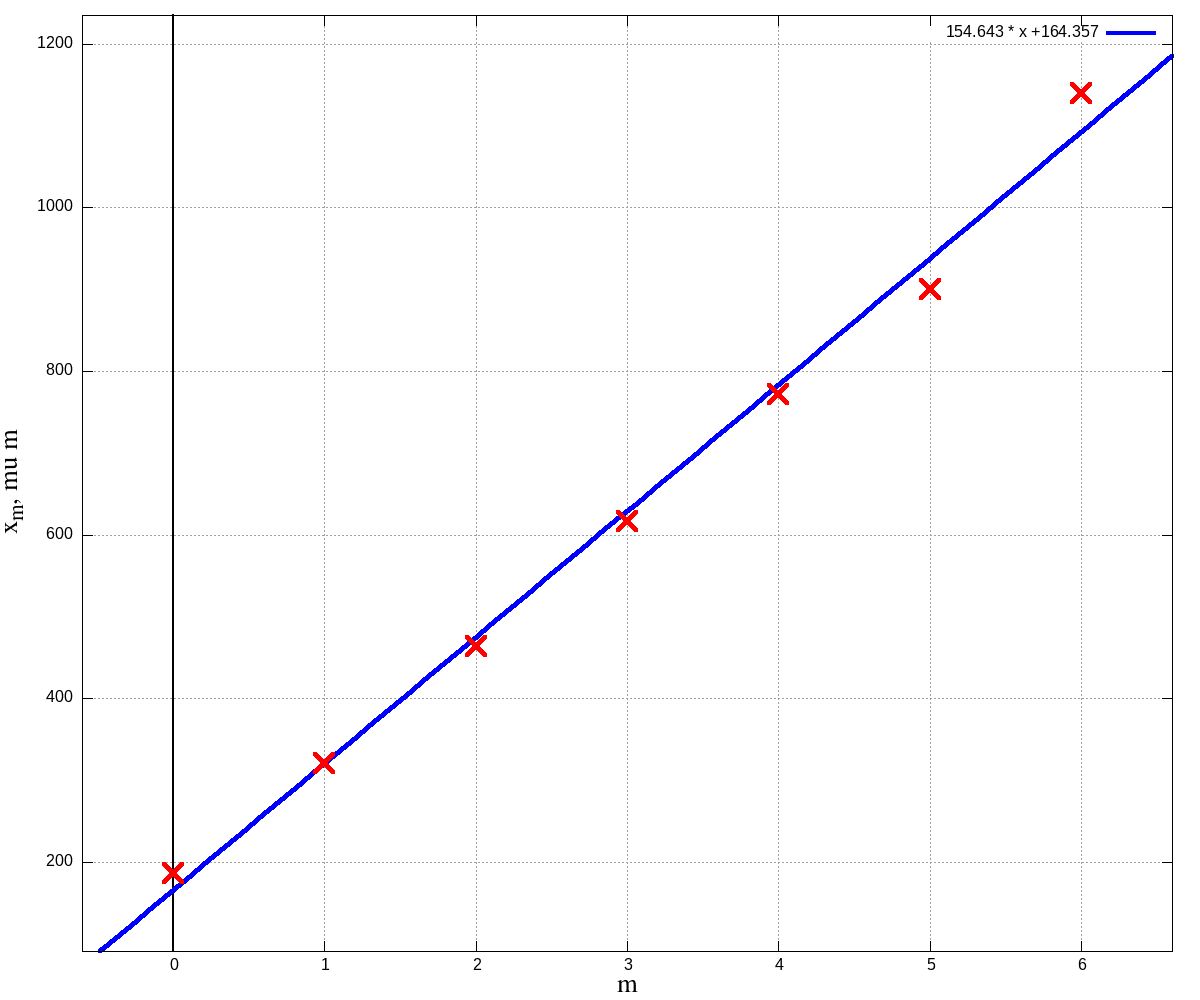
\includegraphics[width=\textwidth]{1140KHz.png}
  \caption{График \(x_m\) от m для \(f = 1.14\; MHz\)}
  \label{fig:1140KHz}
\end{figure}

Получили зависимость вида \(y = kx + b\):
\[ k = (155 \pm 9)\; \mu m \]
\[ b = (161 \pm 14)\; \mu m \]
Из углово-го коэффициента получим, что расстояние между соседними полосами равно:
\[ \Delta x = (155 \pm 9)\; \mu m \]
\[ \Lambda = \frac{f\lambda}{\Delta x} = 1238 \pm 15 \]

\subsection*{\(f = 1.56 \pm 0.005\; MHz\)}
\begin{figure}[H]
  \centering
  \begin{tabular}{|c|c|c|c|c|c|c|c|}
    \hline
    \(m\) & 0 & 1 & 2 & 3 & 4 & 5 & 6\\\hline
    \(x_m,\; (1 \pm 4) \mu m\) & 30 & 220 & 420 & 620 & 832 & 1012 & 1220\\\hline
  \end{tabular}
  \caption{\(f = 1.56\; MHz\)}
\end{figure}

Построим график \(x_m\) от \(m\):
\begin{figure}[H]
  \centering
  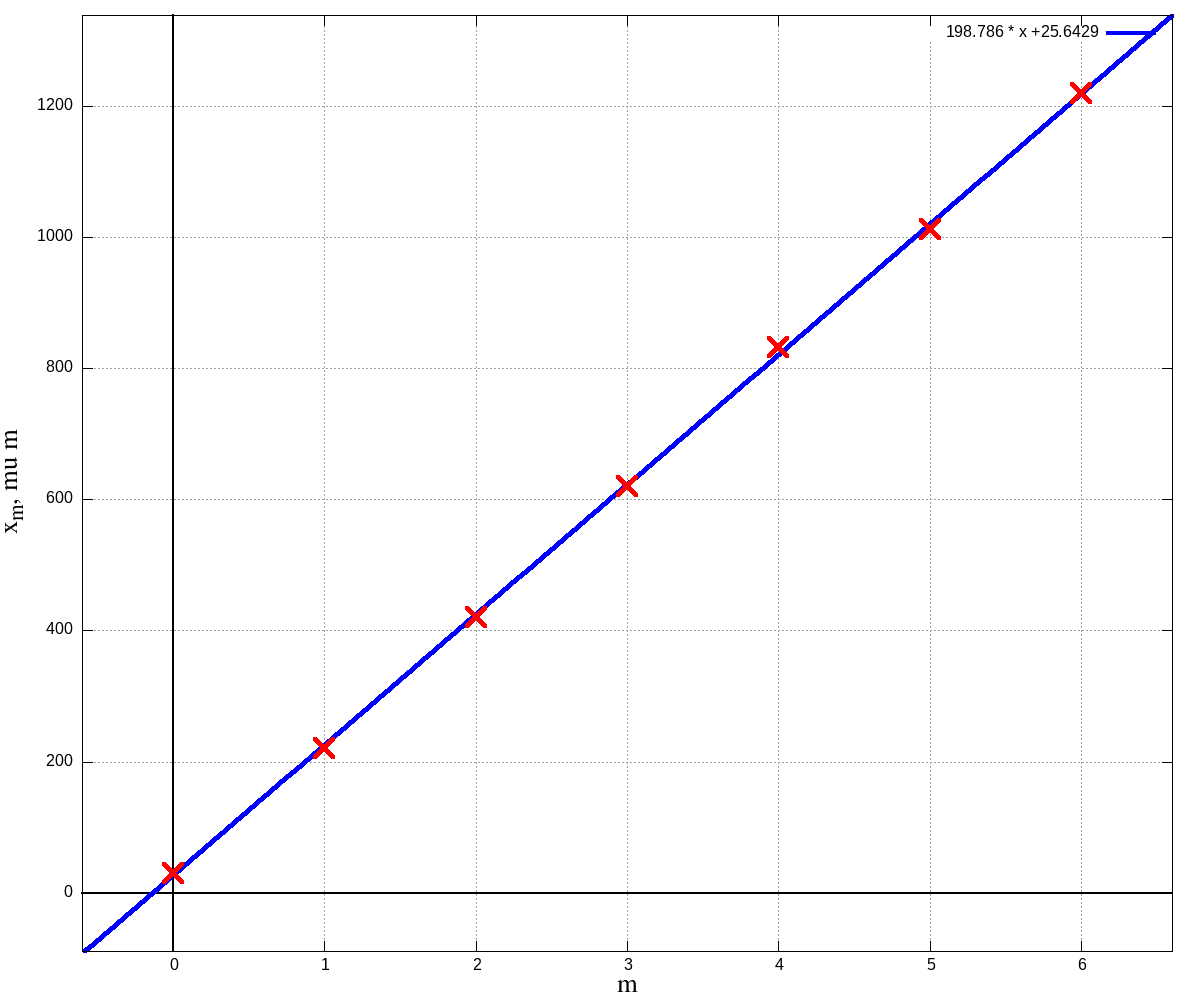
\includegraphics[width=\textwidth]{1560KHz.png}
  \caption{График \(x_m\) от m для \(f = 1.56\; MHz\)}
  \label{fig:1560KHz}
\end{figure}

Получили зависимость вида \(y = kx + b\):
\[ k = (199 \pm 5)\; \mu m \]
\[ b = (26 \pm 6)\; \mu m \]
Из углово-го коэффициента получим, что расстояние между соседними полосами равно:
\[ \Delta x = (199 \pm 5)\; \mu m \]
\[ \Lambda = \frac{f\lambda}{\Delta x} = 946 \pm 16 \]

\subsection*{\(f = 1.84 \pm 0.005\; MHz\)}
\begin{figure}[H]
  \centering
  \begin{tabular}{|c|c|c|c|c|c|c|c|}
    \hline
    \(m\) & 0 & 1 & 2 & 3 & 4\\\hline
    \(x_m,\; (1 \pm 4) \mu m\) & 172 & 400 & 640 & 876 & 1116 \\\hline
  \end{tabular}
  \caption{\(f = 1.84\; MHz\)}
\end{figure}

Построим график \(x_m\) от \(m\):
\begin{figure}[H]
  \centering
  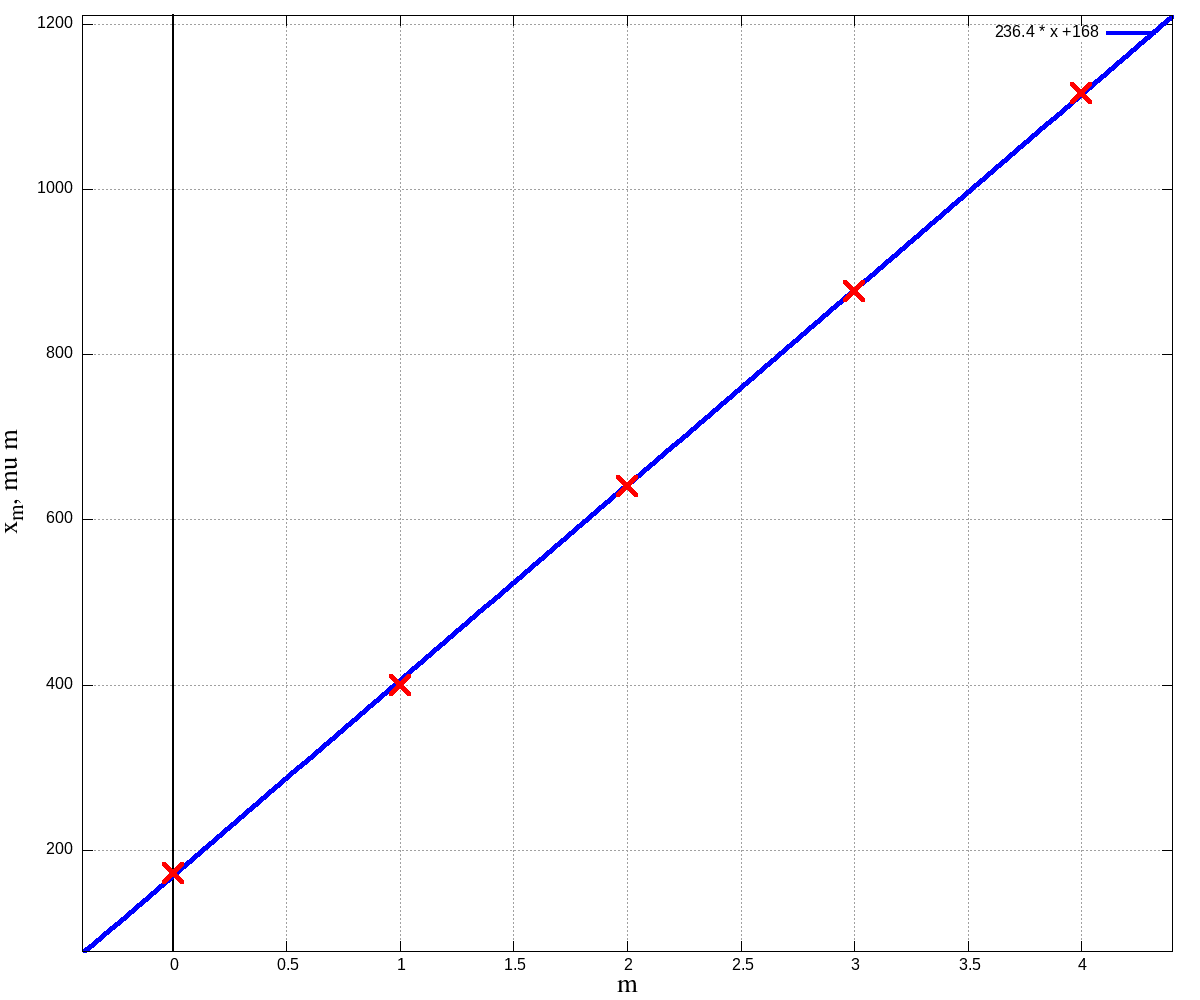
\includegraphics[width=\textwidth]{1840KHz.png}
  \caption{График \(x_m\) от m для \(f = 1.84\; MHz\)}
  \label{fig:1840KHz}
\end{figure}

Получили зависимость вида \(y = kx + b\):
\[ k = (236 \pm 5)\; \mu m \]
\[ b = (168 \pm 6)\; \mu m \]
Из углово-го коэффициента получим, что расстояние между соседними полосами равно:
\[ \Delta x = (236 \pm 5)\; \mu m \]
\[ \Lambda = \frac{f\lambda}{\Delta x} = 813 \pm 16 \]

\subsection{Определение скорости ультразвука методом тёмного поля}
Для перехода к методу тёмного поля (Рис. \ref{fig:dark-scheme}), не смещая микроскоп,
введём микрометрическим винтом в поле зрения микроскопа вертикальную нить.
\begin{figure}[H]
  \centering
  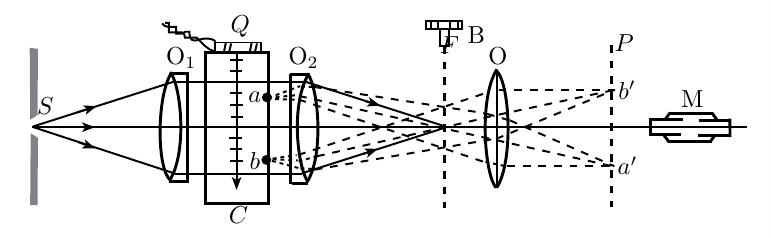
\includegraphics[width=\textwidth]{dark-scheme.png}
  \caption{Наблюдение акустической решётки методом тёмного поля}
  \label{fig:dark-scheme}
\end{figure}

Резкое изображение нити должно совпадать с резким изображением щели. Запишем
соответствующее показание микрометрического винта: 10. Отодвинем микроскоп
и поставьте дополнительную линзу сразу за отсчётным устройством. Опустим в
воду пластинку с миллиметровыми делениями и прижмём её к задней стенке кюветы.
Откроем пошире входную щель. С помощью листа бумаги найдём плоскость, в которой
располагается резкое изображение линейки, созданное двумя линзами. Передвигая
микроскоп в эту точку сфокусируем его на изображении линейки. 

Определите цену деления окулярной шкалы в условиях опыта. Для этого совместим
самые дальние из хорошо видимых в поле зрения милиметровых делений пластинки
с делениями окулярной шкалы и запишем кол-во тех и других делений.
Получим \(10\) делений микроскопа и \(6\) делений линейки. Итого цена деления
микроскопа: \(0.6 \; mm\)

Уберите пластинку из кюветы и уменьшим ширину входной щели. Включим генератор и 
попытаемся увидеть звуковую решётку. Сразу ничего не видно.

Закроем центральный дифракционный максимум вертикальной нитью. Теперь видно
картину:

\begin{figure}[H]
  \centering
  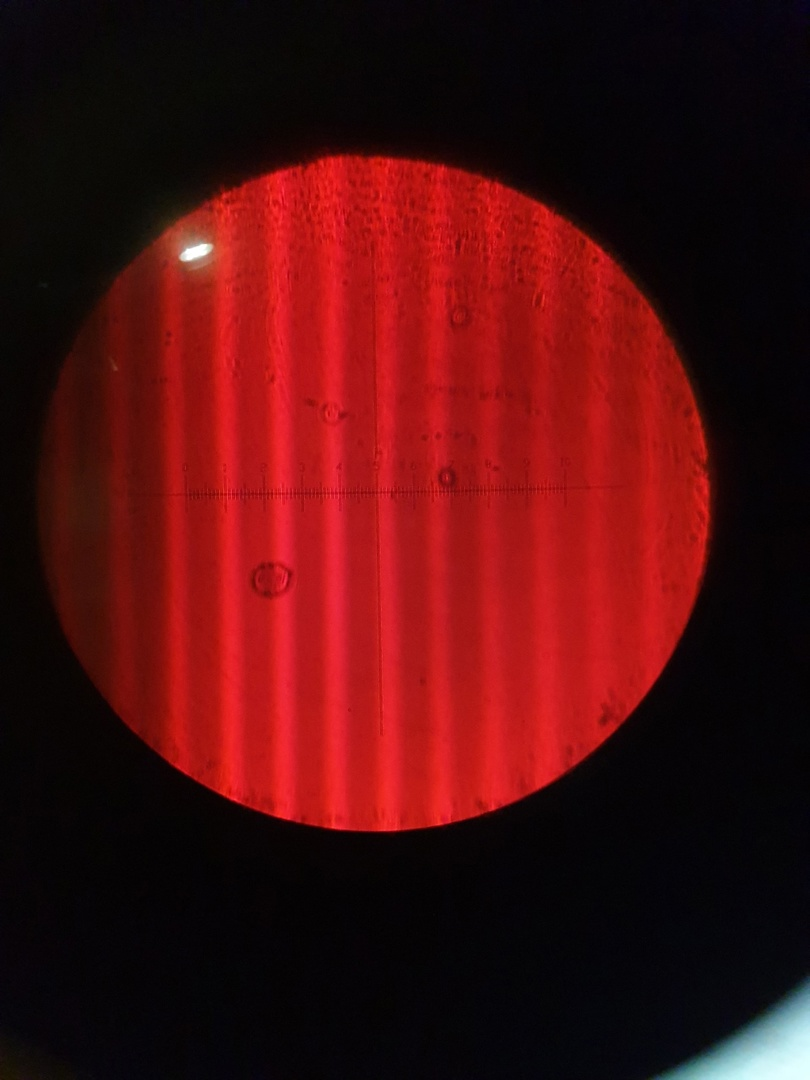
\includegraphics[width=0.5\textwidth]{red-lines.jpg}
  \caption{Звуковая картина}
  \label{fig:red-lines}
\end{figure}

Определим длину УЗ-волны в воде. Для этого с помощью окулярной шкалы измерим
расстояние между самыми дальними из хорошо видимых в поле зрения светлых полос
и просчитаем число промежутков между ними. Проведём измерения для 3 разных
частот.
\begin{figure}[H]
  \centering
  \begin{tabular}{|c|c|c|c|}
    \hline
    \(f, \; MHz\) & 1.16 & 1.53 & 1.85 \\\hline
    \(\lambda,\; \mu m\) & 666 & 545 & 400\\\hline
  \end{tabular}
  \caption{\(f = 1.84\; MHz\)}
\end{figure}

Перемещая проволоку, закроем последовательно минимумы первого, второго и т.д.
порядков. При этом минимумы чередуются с максимумами, ширина полос увеличивается.

\section{Выводы}
В ходе выполнения работы:
\begin{enumerate}
  \item Была изучена дифракция света на синусоидальной акустической решётке.
  \item Была экспериментально оценена скорость звука в воде. Полученное значение
  близко к табличному:
  \[ c_{mes} = (2400 \pm 700)\; m/s\; \textbf{vs}\; c_{th} = 1500\; m/s \]
  \item Были рассчитаны значения длины УЗ-волны. для разных частот ультразвука.
  \item Была получена картина звуковой решётке методом тёмного поля.
\end{enumerate}
\end{document}